\section{MCU}

The MCU on the Camvolution board is used as an I/O-controller, reading from a MicroSD card, configurating the FPGA, and feeding kernel and image data to the FPGA over an EBI bus interface. An EFM32GG is used as the MCU on the Camvolution board, providing 128kB RAM, 1024kB internal flash memory and a range of modules including EBI, USART, GPIO and DMA. The board has headers connected to unused pins on the MCU, making it possible for the MCU to communicate with other devices. Figure \ref{fig:mcuOverview} shows how the components are connected.

\begin{figure}[h!]
    \includegraphics[width=\linewidth]{img/mcu_overview.png}
    \caption{Overview of the components connected to the MCU}
    \label{fig:mcuOverview}
\end{figure}

\subsection{Storage}
Due to the limited size of the MCU non-volatile memory not exceeding 1024kB, an additional larger source of data is necessary. A MicroSD card is used for this storage, as it gives the MCU an external storage of up to 32GB and lets the Camvolution board operate independently without being connected to an external computer.

The code for interfacing the MicroSD card is based on the FAT on SD Card Application Note\cite{an0030}. The MCU communicates with the MicroSD card using SPI transfers with a USART module. FAT32 is used as a filesystem to make reading content from the MicroSD card more manageable, with the trade-off being increased computational overhead for the MCU. This also allows users to add and replace files for the Camvolution board without having to reprogram the MCU.

In the event of the MCU being unable to access the MicroSD card, it is possible to include kernel files and a few small images on the internal flash memory. Functionality for flashing the FPGA from the MCU will be lost because the size of the configuration files exceeds that of the internal flash memory.

The folder structure on the MicroSD card is shown in Table \ref{microsd_folder}.

\begin{table}[h!]
\centering
	\begin{tabular}{ | l | p{10cm} |}
		\hline
		Folder Name & Contents \\ \hline
		binfile & Contains binary configuration files that can be used to program the FPGA to alter its behaviour. \\ \hline
		image & Contains images that can be fed to the FPGA. Serves as a backup for the camera input. Supports 24-bit BMP files and 24-bit raw image data. \\ \hline
		kernel & Contains different kernels used for convolution. \\ \hline
	\end{tabular}
	\caption{MicroSD card folder structure}
	\label{microsd_folder}
\end{table}


\subsection{FPGA Configuration}
When the Camvolution board is powered up the FPGA will not contain a configuration. To be able to use the FPGA properly, the MCU has to program it with one of the binfiles from the storage. Pins between the MCU and the FPGA are connected according to Slave Serial as described in Spartan 6 Configuration User Guide\cite{ug380} page 28. This configuration scheme relies on sending a binfile as a serial data stream using a clk pin and a single data pin. The MCU is able to reset the configuration of the FPGA at any time by setting the program pin low. Configuration status pins set by the FPGA informs the MCU if it is ready to be programmed, if an error occured while programming or if the FPGA has succesfully programmed. 

The FPGA can also be reprogrammed later. For example when using kernels of different sizes, a configuration optimized for a specific size can be configurated on the FPGA.


\subsection{Kernels}
The kernel files consists of 8-bit values. The first byte tells the size of the kernel. For a 3x3 kernel the size will be 9. This limits us to a maximum size of 15x15 kernels. The next byte is the divisor, which is used for averaging filters. The rest of the bytes in the files are the elements of the kernel.


\subsection{External Bus Interface}
\begin{wrapfigure}[14]{r}{6cm}
    \centering
    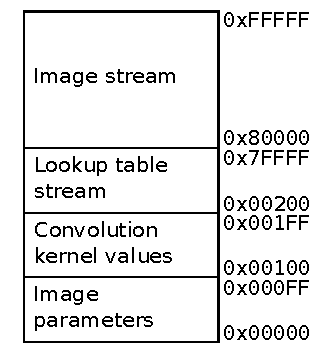
\includegraphics[]{img/EbiAddressSpace.pdf}
    \caption{EBI Address Space}
    \label{fig:EbiAddressSpace}
\end{wrapfigure}
The FPGA and the MCU is connected through an EBI bus.
This interface is supported natively by the MCU and can therefore be handled by its built-in direct memory access (DMA) unit, which hopefully makes streaming video from the MCU faster, more reliable and easier to implement.

In addition to streaming video, the MCU should also control the operation of Daisy.
To accomplish this, we utilize the large address space available.
An overview can be seen in figure \ref{fig:EbiAddressSpace}.

\subsubsection{Daisy Configuration}
Configuration values for Daisy have their own memory addresses so that configuring daisy is only a matter of saving the correct values to the correct addresses.

Note that the amount of space allocated to each group of options in figure \ref{fig:EbiAddressSpace} is more than needed.
This simplifies the process of adding more configuration options if required at a later point.

\subsubsection{Streaming Data}
Some data is of unknown or unlimited length. This data is streamed to daisy by reusing the same addresses several times.
By assigning a large block of the memory space to each data stream, we can utilize the DMA without having to worry about unintendedly overwriting configuration values.

The reuse of addresses also provides a natural sync point for the video stream;
each write to the first address of the address space reserved for streaming video is assumed to be a \textit{frame sync}, which signals the start of a new frame.
This makes the system less fragile as Daisy can catch up with the data stream should it ever end up being out of sync.
